%% ============================================================
%% 分片 17：原文第 6 节「Loop and Line Operators」（原文 glshort.tex 起于第 4483 行）
%% 由 tools/harvmac2tex.py 从 arXiv 源码（hep-th/0604151v3）自动生成。
%% 只译英文散文；公式、编号、\label、\cite 一律不改。
%% ============================================================

\subsection{Compactification To Two Dimensions}

\label{sec:comptwo}

We now want to consider the interpretation of loop or line
operators after compactification to two dimensions.  We set
$M=\Sigma\times C$, with $\Sigma$ and $C$ being Riemann surfaces.
Thinking of $\Sigma$ as being much bigger than $C$, we want to ask
what loop operators look like in an effective two-dimensional
theory on $\Sigma$. To begin with, we assume that $\Sigma$ has no
boundary.

\begin{figure}[htbp]
\centering
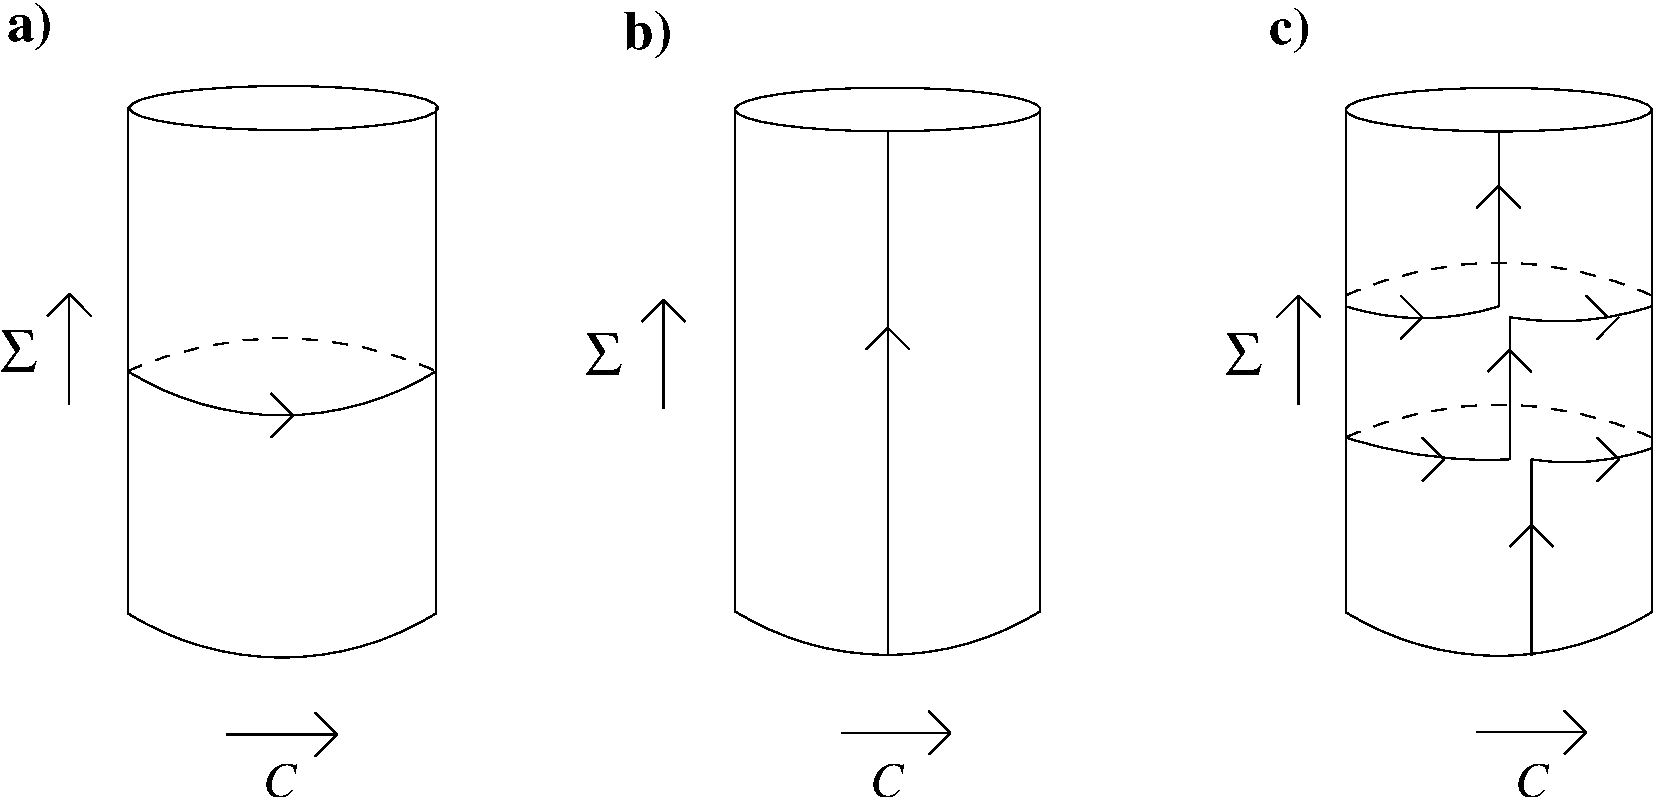
\includegraphics[width=0.75\linewidth]{figures/gla4-1.png}
\caption{A schematic depiction of the four-manifold $\Sigma\times C$, with $\Sigma$ running vertically and $C$ horizontally. (a) A Wilson line that propagates in the $C$ direction. (b) A Wilson line that propagates in the $\Sigma$ direction. (c) A Wilson line that propagates in $\Sigma$, except at two moments at which it loops around one-cycles in $C$.（原文 Fig.~4）}
\label{fig:namp-four}  % 原文 \ifig\namp 同名重复（§6 Fig.~4 与 §8 Fig.~11），此处改名以免冲突
\end{figure}
 Several cases can be
distinguished.  One case  (\namp(a)) is a loop of the form ${{\cal
S}}=p\times {{\cal S}}'$, where $p$ is a point in $\Sigma$ and
${{\cal S}}'$ is a loop in $C$. Clearly, an operator supported on
a loop of this kind simply looks like a pointlike local operator
in the effective theory on $\Sigma$.  All ordinary quantum field
theories and many TQFT's have such local operators, so in this
example, the loop operator, after compactification, turns into
something fairly ordinary in the effective theory on $\Sigma$.

The opposite case (\namp(b)) is ${{\cal S}}={{\cal S}}''\times q$,
with ${{\cal S}}''$ a loop in $\Sigma$ and $q$ a point in $C$.
Here the loop operator remains as a loop operator in the effective
two-dimensional theory.

The general case, of course, is a curve ${{\cal S}}$ that
propagates non-trivially in both $\Sigma$ and $C$.  Any such curve
is homotopic to a curve that propagates first on $\Sigma$, then on
$C$, then on $\Sigma$, and so on, as indicated in \namp(c). Let
$\bar {{\cal S}}$ be the projection of ${{\cal S}}$ to $\Sigma$. A
loop operator on ${{\cal S}}$ reduces in the effective theory on
$\Sigma$ to a loop operator on $\bar {{\cal S}}$ with local
operators inserted at distinguished points on $\bar {{\cal S}}$,
namely the points where ${{\cal S}}$ propagates around $C$. We
will momentarily describe a different interpretation of such a
loop operator.

\begin{figure}[htbp]
\centering
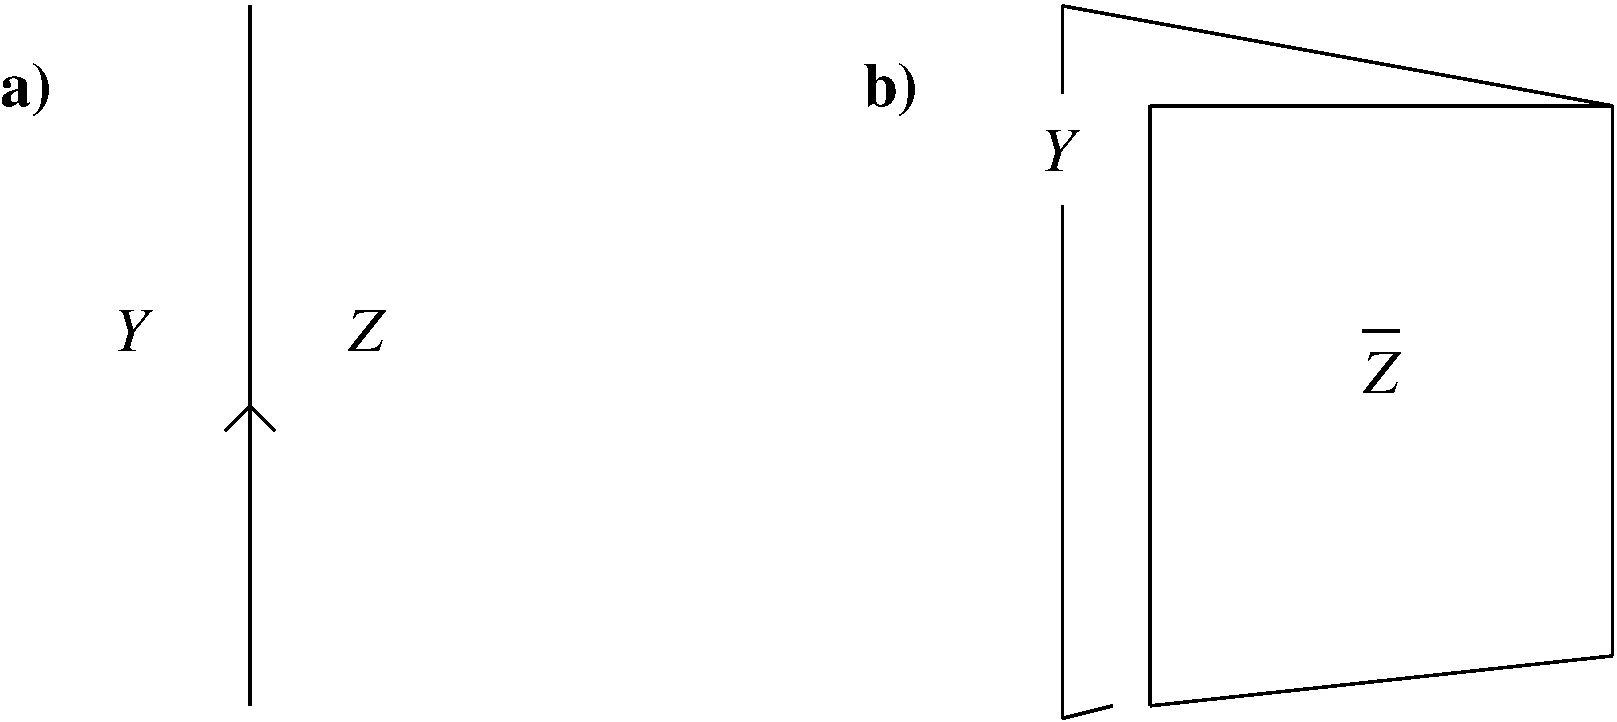
\includegraphics[width=0.75\linewidth]{figures/gla4-2.png}
\caption{(a) A line operator dividing the plane into two regions, labeled by theories $Y$ and $Z$. (b) A folded version of the same picture, interpreted in terms of theory $Y\times \bar Z$ on a half-plane; the boundary is labeled by a $(Y,Z)$-brane.（原文 Fig.~5）}
\label{fig:tonamp}
\end{figure}
 The essential point is
clearly to understand the meaning of a loop or line operator in
two dimensions.  Here we should note that a two-manifold is
locally divided by a one-manifold into two disjoint regions.
Hence, a loop or line operator might  produce a long-range effect;
the couplings in the two-dimensional effective theory  might be
different on the two sides.  (How Wilson and 't Hooft line
operators can have such an effect is discussed in section
第~\ref{sec:wilbranes}~节.) This possibility is incorporated in \tonamp(a), where
we sketch a two-dimensional line operator that divides the plane
into two regions labeled by two distinct theories, $Y$ and $Z$.

To put this situation in a more familiar framework, we can use a
``folding'' trick (see for example \cite{ref93,ref94,ref95}).  At the cost of reversing the
orientation of region $Z$ to get what we will call theory $\bar
Z$, we can ``fold'' \tonamp(a) to get a similar figure in which
regions $Y$ and $Z$ are on the same side and end at the location
of the line operator (\tonamp(b)).

What we have now from an abstract point of view is a boundary
condition in the tensor product theory $Y\otimes \bar Z$.  For
purposes of this paper, by a ``brane,'' in general, we simply mean
a local boundary condition in a quantum field theory.  (In other
words, our branes are all $D$-branes.) We will refer to branes of
the product theory $Y\otimes \bar Z$ as $(Y,Z)$-branes. So the
line operator reduces in two dimensions to a $(Y,Z)$-brane.

Now we can also understand \namp(c) a little better. We previously
interpreted this configuration in terms of a line operator with
local operators inserted on it.  After folding, the effective
two-dimensional theory is formulated on a Riemann surface $\Sigma$
with boundary and with local operators inserted on the boundary.
Their existence is characteristic of brane physics; in general,
for any brane, there is a certain space of local operators that
can be inserted on a boundary component of $\Sigma$ that is
labeled by that brane.

\begin{figure}[htbp]
\centering
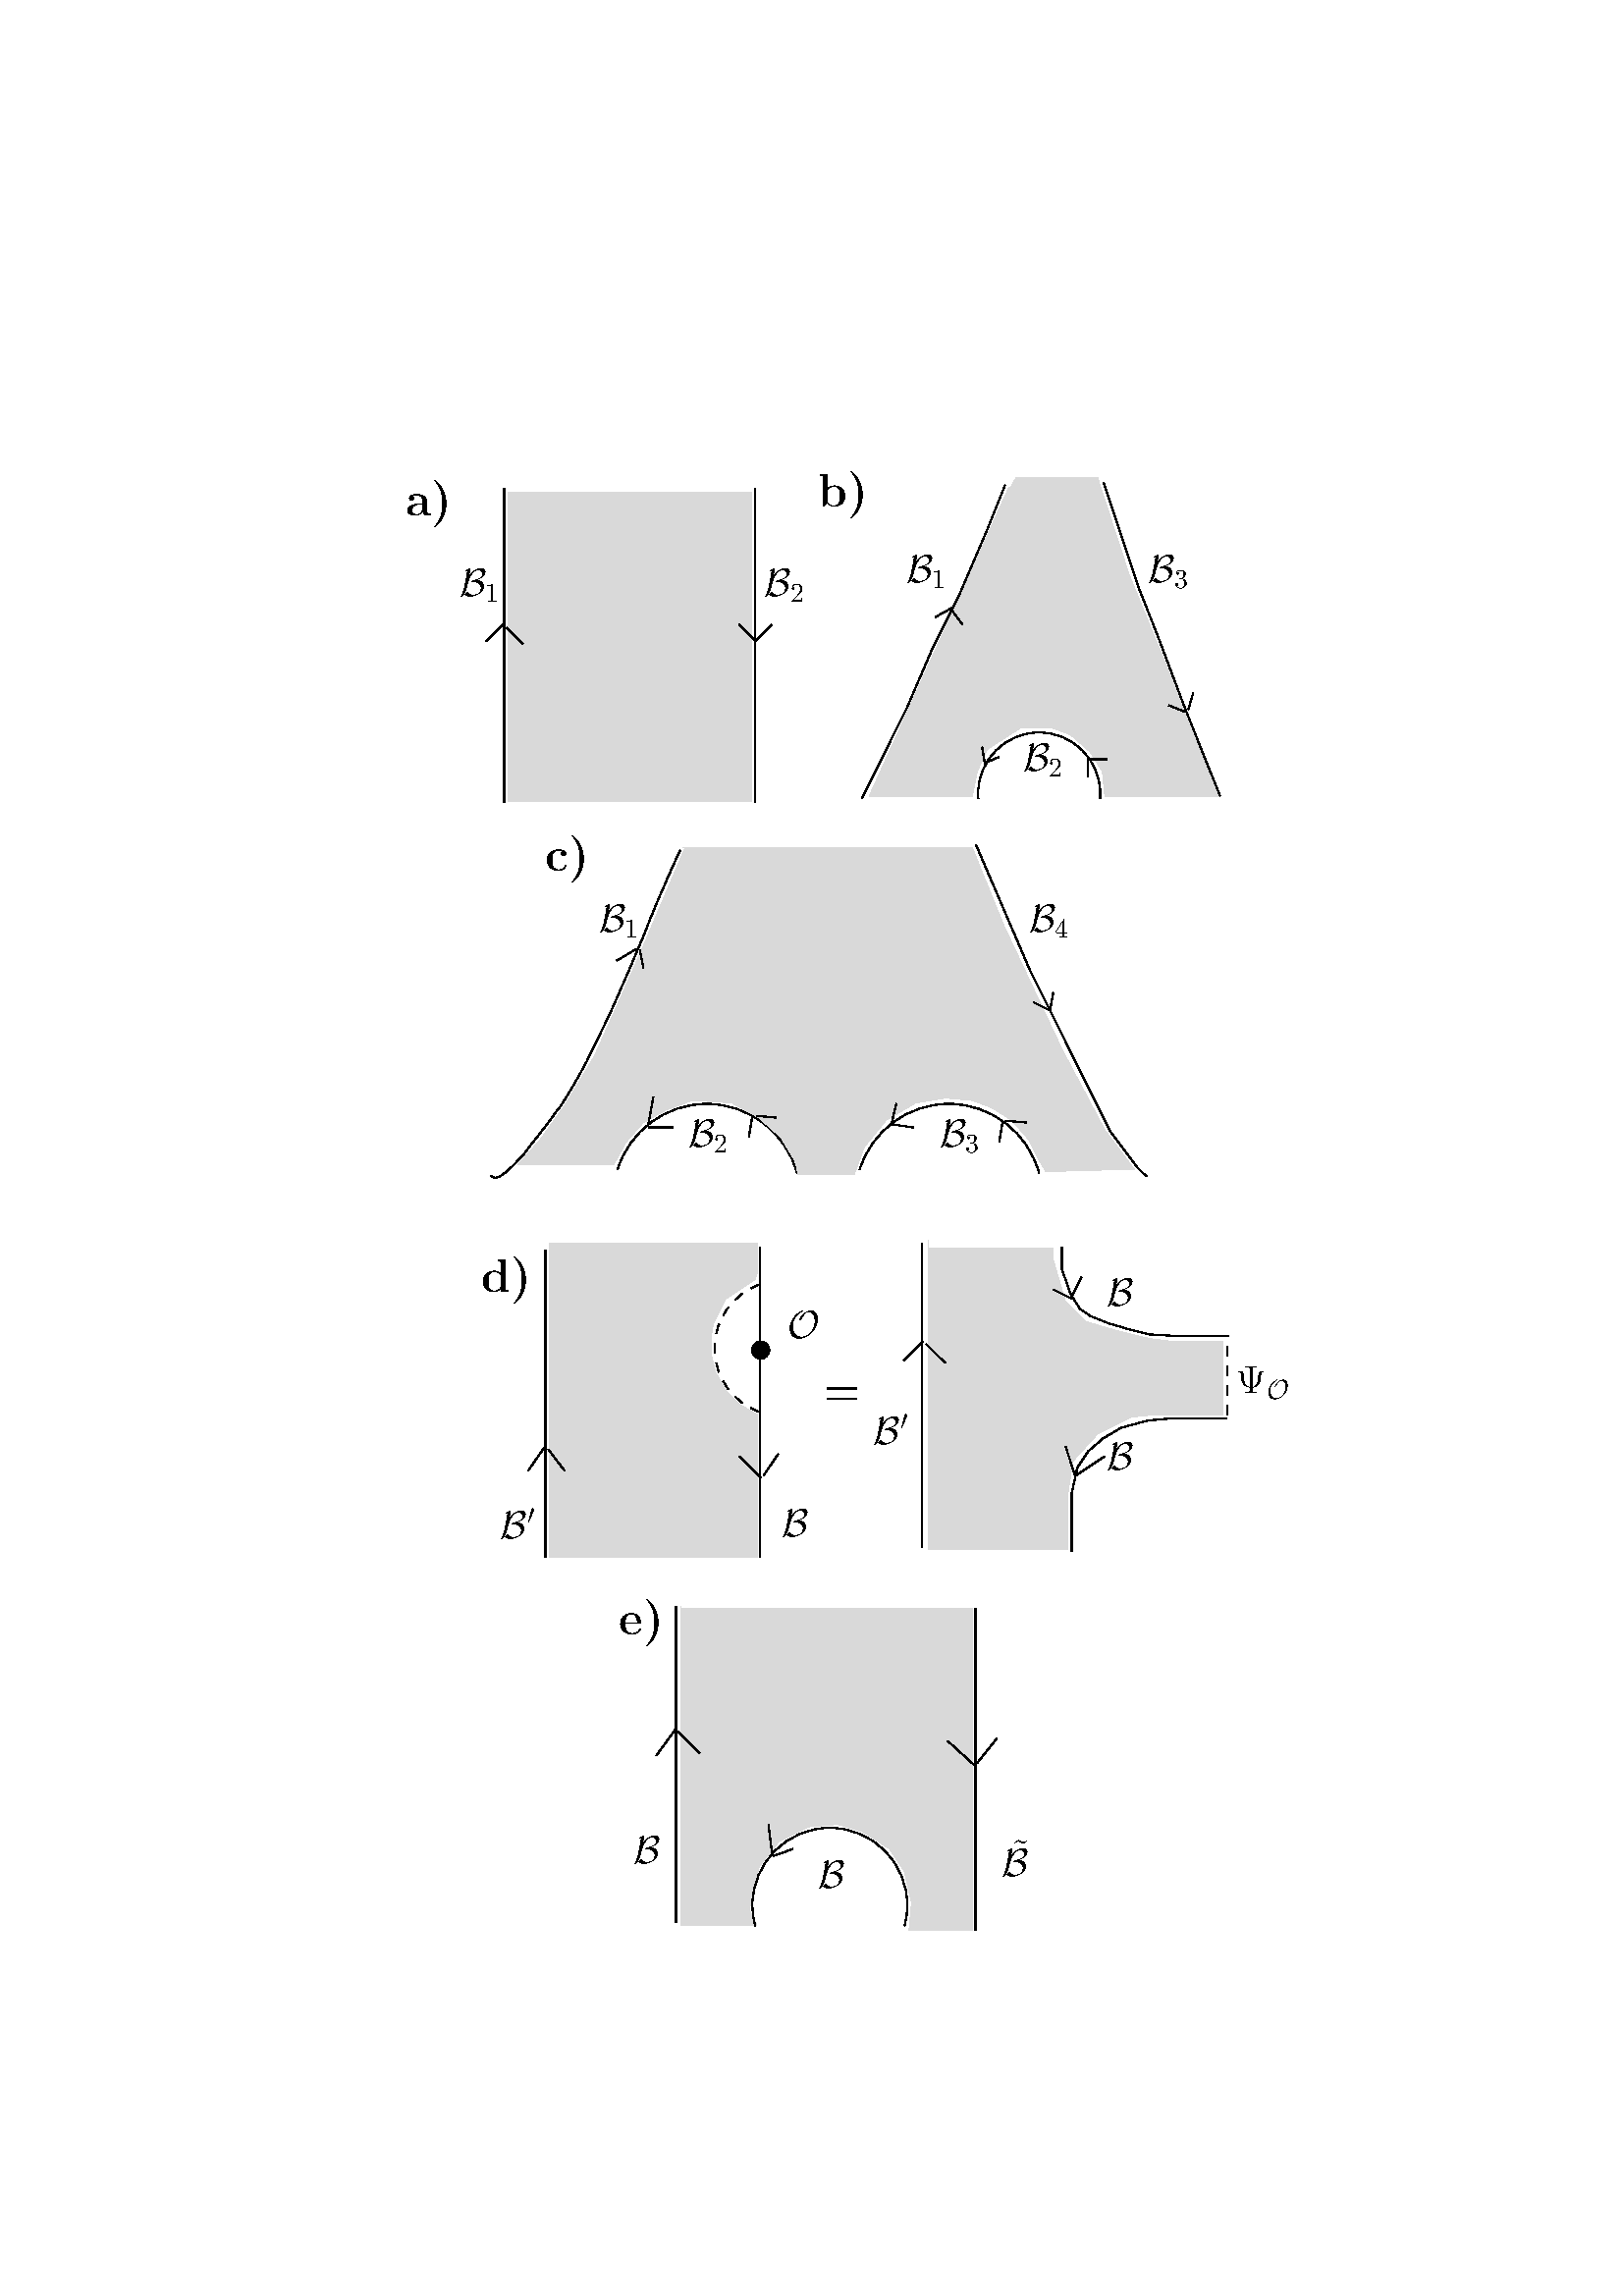
\includegraphics[width=0.75\linewidth]{figures/gla4-3.png}
\caption{(a) The space of $({\cal B}_1,{\cal B}_2)$ strings. (b) Joining of strings to make a product ${\cal H}_{{\cal B}_1,{\cal B}_2}\otimes {\cal H}_{{\cal B}_2,{\cal B}_3}\to {\cal H}_{{\cal B}_1,{\cal B}_3}$. (c) The associativity relation that comes by joining three strings. (d) The space of local operators ${\EUO}$ that can be inserted on a boundary labeled by a brane ${\cal B}$ is the same as the space ${\cal H}_{{\cal B},{\cal B}}$. To see this, we perform the path integral in a small region around the insertion point of ${\EUO}$ (the unshaded region on the left) to get a physical state $\Psi_{\EUO}$ that can be inserted on the dotted line to reproduce the effects of ${\EUO}$. The resulting picture can be put in the form shown on the right. (e) For every ${\cal B}$ and $\tilde{\cal B}$, the space ${\cal H}_{{\cal B},\tilde{\cal B}}$ is a module for the algebra ${\cal H}_{{\cal B},{\cal B}}$.（原文 Fig.~6）}
\label{fig:dunamp}
\end{figure}

 Let us recall how to characterize such local operators. This will also help us
recall a few basic facts about branes. For every two-dimensional
quantum field theory $X$ and pair of branes ${\cal B}_1$ and
${\cal B}_2$, one defines a vector space ${\cal H}_{{\cal
B}_1,{\cal B}_2}$ of $({\cal B}_1,{\cal B}_2)$ strings. In unitary
quantum field theory, these spaces are Hilbert spaces; even
without unitarity, ${\cal H}_{{\cal B}_1,{\cal B}_2}$ is dual to
${\cal H}_{{\cal B}_2,{\cal B}_1}$. One defines ${\cal H}_{{\cal
B}_1,{\cal B}_2}$ by quantizing the theory $X$ on
$\Sigma=\Bbb{R}\times I$, with $I$ a unit interval whose ends are
labeled respectively by ${\cal B}_1$ and ${\cal B}_2$
(\dunamp(a)). ${\cal H}_{{\cal B}_1,{\cal B}_2}$ is also called
the space of physical states of the theory with the given boundary
conditions at the two ends of $I$.

Now in topological field theory, there are for any branes ${\cal
B}_1,{\cal B}_2,$ and $ {\cal B}_3$ natural maps ${\cal H}_{{\cal
B}_1,{\cal B}_2}\otimes {\cal H}_{{\cal B}_2,{\cal B}_3}\to {\cal
H}_{{\cal B}_1,{\cal B}_3}$ defined by joining Riemann surfaces
together (\dunamp(b)).  (In two-dimensional quantum field theory
without topological invariance, one must take into account the
metrics or conformal structures of the surfaces, as a result of
which an analogous discussion leads to the operator product
expansion.) These maps obey the obvious associativity relation,
which says that when three strings are joined  (\dunamp(c)), one
does not have to say which two joined first. In particular,
setting all the branes ${\cal B}_i$ equal to ${\cal B}$, we find
that ${\cal H}_{{\cal B},{\cal B}}$ always has the natural
structure of an associative algebra.

In fact, in TQFT, the space of local operators ${\EUO}$ that can
be inserted on a a boundary labeled by a brane ${\cal B}$ is the
same as ${\cal H}_{{\cal B},{\cal B}}$, since (\dunamp(d)) a
``cutting'' operation applied near such an ${\EUO}$ reveals an
element of ${\cal H}_{{\cal B},{\cal B}}$. By similar reasoning
(\dunamp(e)), we find that, for any ${\cal B}$ and  $ \tilde{\cal
B}$, ${\cal H}_{{\cal B}, \tilde{\cal B}}$ always has a natural
structure of left ${\cal H}_{{\cal B},{\cal B}}$-module.
Similarly, it has a natural structure of right ${\cal H}_{\tilde
{\cal B},\tilde{\cal B}}$ module. Indeed, ${\cal H}_{{\cal B},
\tilde{\cal B}}$ is a $({\cal H}_{{\cal B},{\cal B}},{\cal
H}_{\tilde{\cal B},\tilde{\cal B}})$ bimodule. This means simply
that one can act with ${\cal H}_{{\cal B},{\cal B}}$ by attaching
a string on the left, or by ${\cal H}_{\tilde{\cal B},\tilde{\cal
B}}$ by attaching a string on the right, and moreover these two
actions commute.
